\subsection{Database}
	All'interno dell'architettura sono utilizzati:
	\begin{itemize}
		\item un database relazionale, \glock{PostgreSQL}, che viene usato per il salvataggio delle configurazioni dei gateway, delle informazioni di utenti ed enti, oltre alle impostazioni dei grafici creati dagli utenti stessi;
		\item un database non relazionale, \glock{Timescale}, che viene usato per salvare i dati inviati dai dispositivi, le logs degli eventi e gli alert con i valori anomali rilevati. 
	\end{itemize}
	Entrambi i database sono rilasciati tramite dockerfile, tramite il quale ne viene effettuata una prima configurazione.
	\subsubsection{Timescale}
	La struttura del database non relazionale è la seguente:
	\begin{itemize}
		\item Sensors
		\begin{itemize}
			\item time: timestamptz
			\item real\_sensor\_id: integer
			\item real\_device\_id: integer
			\item gateway\_name: text
			\item value: double
		\end{itemize}
		\item Logs
		\begin{itemize}
			\item time: timestamptz
			\item user\_id: integer
			\item ip\_address: varchar
			\item operation: text
			\item data: text
		\end{itemize}
	\end{itemize}
	\subsubsection{PostgreSql}
	La struttura del database SQL è rappresentata nello schema logico sottostante:
		
			\begin{landscape}
			\begin{figure}[H]
				\centering
				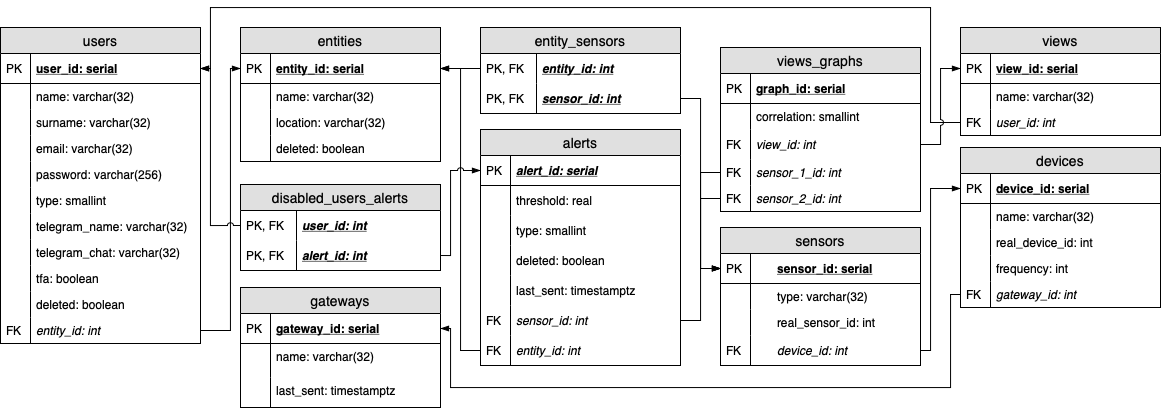
\includegraphics[scale=0.600]{res/images/DATABASE/ER_Modificato.png}
				\caption{Diagramma logico del database relazionale}
				\label{Diagramma 9}
			\end{figure}
			\end{landscape}
	\subsubsection{Estensioni}
		\paragraph{Duplicazione dei dati nel database Timescale}
			Per aggiungere un fattore di duplicazione ai dati è necessario modificare il file docker-compose.yml inserendo un nuovo servizio: il servizio che si andrà a duplicare sarà quello di \glock{Timescale}, che sarà copiato e modificato.
			\newline
			Risulterà infatti necessario modificare il nome del servizio e del container, la mappatura delle porte (prestando attenzione a mantenere la porta interna specificata) ed infine i volumi.
			\newline
			Per effettuare la persistenza dei dati sarà infine necessario inserire il nuovo volume mappato all'interno di "volumes".
			Conclusa questa procedura sarà possibile inserire il nuovo database all'interno della componente DataCollector, specificando il corretto indirizzo.

		\paragraph{Modifica impostazioni d'accesso ai database}	
			Per modificare le impostazioni di accesso ai database è necessario modificare le variabili d'ambiente all'interno dei rispettivi Dockerfile.		